\begin{enumerate}
	\item In an equilateral $\triangle ABC, D$ is a point on side $BC$ such that $ BD =\frac{1}{3}BC$. Prove that $9(AD)^2 = 7(AB)^2$.
	\hfill\brak{10, 2018}
\item Prove that the area of an equilateral triangle described on one side of the square is equal to half of the area of the equilateral triangle described on one of its diagonal.
	\hfill\brak{10, 2018}\item If the areas of two similar triangles are equal, prove that they are congruent.
\hfill\brak{10, 2018}
\item In \figref{fig:rightangled4}, $BN$ and $CM$ are medians of a $\triangle ABC$ right-angled at $A$. Prove that \begin{align*}4(BN^2 +CM^2) = 5BC^2\end{align*} 
\begin{figure}[H]
\centering
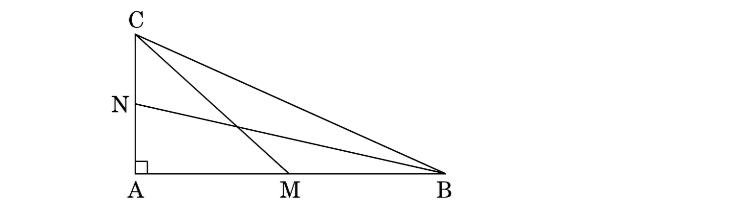
\includegraphics[width=\columnwidth]{cbse/figs/rightangled}
\caption{}
\label{fig:rightangled4}
\end{figure}
%
\hfill\brak{10, 2022}\item If $A$, $B$ and $C$ are interior angles of $ \triangle ABC$, then show that
\hfill\brak{10, 2020} 
	\begin{align*}
	    \cos \brak{\frac{B + C}{2}}=\sin \brak{\frac{A}{2}}
	\end{align*}
%      
\item  In $\triangle ABC$, right-angled at $A$, if $AB=7 cm$ and $AC=24 cm$, then find $\sin B$
and $\tan C$.
%

\hfill\brak{10, 2021}\item Two angles of a triangle are  $\cot^{-1}2$ and $\cot^{-1}3$. The third angle of the
triangle is \rule{1cm}{0.1pt}.
%
\hfill\brak{12, 2021}
%
\item $A$, $B$ and $C$ are interior angles of a triangle $ABC$. Show that
\hfill\brak{10, 2019}
\begin{enumerate}
\item  $\sin$ $ \brak{{\frac {B+C}{2}}} = \cos {\frac {A}{2}}$
\item  If $\angle A = 90 \degree$, then find the value of $\tan \brak{{\frac{B+C}{2}}}$.
\end{enumerate} 
%
	\item In $\triangle$ $ABC$, $AB = {4\sqrt{3}}$ cm, $AC = 8 cm$ and $BC = 4 cm$. The angle $B$ is
	\hfill\brak{10, 2021}
	\begin{multicols}{4}
				\begin{enumerate}
\item $120\degree$
\item $90\degree$
\item $60\degree$
\item $45\degree$
				\end{enumerate}
\end{multicols}
%
\end{enumerate}
